% Generated by Sphinx.
\def\sphinxdocclass{report}
\documentclass[letterpaper,10pt,english]{sphinxmanual}
\usepackage[utf8]{inputenc}
\DeclareUnicodeCharacter{00A0}{\nobreakspace}
\usepackage{cmap}
\usepackage[T1]{fontenc}
\usepackage{babel}
\usepackage{times}
\usepackage[Bjarne]{fncychap}
\usepackage{longtable}
\usepackage{sphinx}
\usepackage{multirow}


\title{matchApp Documentation}
\date{June 23, 2016}
\release{2}
\author{Grupo5}
\newcommand{\sphinxlogo}{}
\renewcommand{\releasename}{Release}
\makeindex

\makeatletter
\def\PYG@reset{\let\PYG@it=\relax \let\PYG@bf=\relax%
    \let\PYG@ul=\relax \let\PYG@tc=\relax%
    \let\PYG@bc=\relax \let\PYG@ff=\relax}
\def\PYG@tok#1{\csname PYG@tok@#1\endcsname}
\def\PYG@toks#1+{\ifx\relax#1\empty\else%
    \PYG@tok{#1}\expandafter\PYG@toks\fi}
\def\PYG@do#1{\PYG@bc{\PYG@tc{\PYG@ul{%
    \PYG@it{\PYG@bf{\PYG@ff{#1}}}}}}}
\def\PYG#1#2{\PYG@reset\PYG@toks#1+\relax+\PYG@do{#2}}

\expandafter\def\csname PYG@tok@gd\endcsname{\def\PYG@tc##1{\textcolor[rgb]{0.63,0.00,0.00}{##1}}}
\expandafter\def\csname PYG@tok@gu\endcsname{\let\PYG@bf=\textbf\def\PYG@tc##1{\textcolor[rgb]{0.50,0.00,0.50}{##1}}}
\expandafter\def\csname PYG@tok@gt\endcsname{\def\PYG@tc##1{\textcolor[rgb]{0.00,0.27,0.87}{##1}}}
\expandafter\def\csname PYG@tok@gs\endcsname{\let\PYG@bf=\textbf}
\expandafter\def\csname PYG@tok@gr\endcsname{\def\PYG@tc##1{\textcolor[rgb]{1.00,0.00,0.00}{##1}}}
\expandafter\def\csname PYG@tok@cm\endcsname{\let\PYG@it=\textit\def\PYG@tc##1{\textcolor[rgb]{0.25,0.50,0.56}{##1}}}
\expandafter\def\csname PYG@tok@vg\endcsname{\def\PYG@tc##1{\textcolor[rgb]{0.73,0.38,0.84}{##1}}}
\expandafter\def\csname PYG@tok@m\endcsname{\def\PYG@tc##1{\textcolor[rgb]{0.13,0.50,0.31}{##1}}}
\expandafter\def\csname PYG@tok@mh\endcsname{\def\PYG@tc##1{\textcolor[rgb]{0.13,0.50,0.31}{##1}}}
\expandafter\def\csname PYG@tok@cs\endcsname{\def\PYG@tc##1{\textcolor[rgb]{0.25,0.50,0.56}{##1}}\def\PYG@bc##1{\setlength{\fboxsep}{0pt}\colorbox[rgb]{1.00,0.94,0.94}{\strut ##1}}}
\expandafter\def\csname PYG@tok@ge\endcsname{\let\PYG@it=\textit}
\expandafter\def\csname PYG@tok@vc\endcsname{\def\PYG@tc##1{\textcolor[rgb]{0.73,0.38,0.84}{##1}}}
\expandafter\def\csname PYG@tok@il\endcsname{\def\PYG@tc##1{\textcolor[rgb]{0.13,0.50,0.31}{##1}}}
\expandafter\def\csname PYG@tok@go\endcsname{\def\PYG@tc##1{\textcolor[rgb]{0.20,0.20,0.20}{##1}}}
\expandafter\def\csname PYG@tok@cp\endcsname{\def\PYG@tc##1{\textcolor[rgb]{0.00,0.44,0.13}{##1}}}
\expandafter\def\csname PYG@tok@gi\endcsname{\def\PYG@tc##1{\textcolor[rgb]{0.00,0.63,0.00}{##1}}}
\expandafter\def\csname PYG@tok@gh\endcsname{\let\PYG@bf=\textbf\def\PYG@tc##1{\textcolor[rgb]{0.00,0.00,0.50}{##1}}}
\expandafter\def\csname PYG@tok@ni\endcsname{\let\PYG@bf=\textbf\def\PYG@tc##1{\textcolor[rgb]{0.84,0.33,0.22}{##1}}}
\expandafter\def\csname PYG@tok@nl\endcsname{\let\PYG@bf=\textbf\def\PYG@tc##1{\textcolor[rgb]{0.00,0.13,0.44}{##1}}}
\expandafter\def\csname PYG@tok@nn\endcsname{\let\PYG@bf=\textbf\def\PYG@tc##1{\textcolor[rgb]{0.05,0.52,0.71}{##1}}}
\expandafter\def\csname PYG@tok@no\endcsname{\def\PYG@tc##1{\textcolor[rgb]{0.38,0.68,0.84}{##1}}}
\expandafter\def\csname PYG@tok@na\endcsname{\def\PYG@tc##1{\textcolor[rgb]{0.25,0.44,0.63}{##1}}}
\expandafter\def\csname PYG@tok@nb\endcsname{\def\PYG@tc##1{\textcolor[rgb]{0.00,0.44,0.13}{##1}}}
\expandafter\def\csname PYG@tok@nc\endcsname{\let\PYG@bf=\textbf\def\PYG@tc##1{\textcolor[rgb]{0.05,0.52,0.71}{##1}}}
\expandafter\def\csname PYG@tok@nd\endcsname{\let\PYG@bf=\textbf\def\PYG@tc##1{\textcolor[rgb]{0.33,0.33,0.33}{##1}}}
\expandafter\def\csname PYG@tok@ne\endcsname{\def\PYG@tc##1{\textcolor[rgb]{0.00,0.44,0.13}{##1}}}
\expandafter\def\csname PYG@tok@nf\endcsname{\def\PYG@tc##1{\textcolor[rgb]{0.02,0.16,0.49}{##1}}}
\expandafter\def\csname PYG@tok@si\endcsname{\let\PYG@it=\textit\def\PYG@tc##1{\textcolor[rgb]{0.44,0.63,0.82}{##1}}}
\expandafter\def\csname PYG@tok@s2\endcsname{\def\PYG@tc##1{\textcolor[rgb]{0.25,0.44,0.63}{##1}}}
\expandafter\def\csname PYG@tok@vi\endcsname{\def\PYG@tc##1{\textcolor[rgb]{0.73,0.38,0.84}{##1}}}
\expandafter\def\csname PYG@tok@nt\endcsname{\let\PYG@bf=\textbf\def\PYG@tc##1{\textcolor[rgb]{0.02,0.16,0.45}{##1}}}
\expandafter\def\csname PYG@tok@nv\endcsname{\def\PYG@tc##1{\textcolor[rgb]{0.73,0.38,0.84}{##1}}}
\expandafter\def\csname PYG@tok@s1\endcsname{\def\PYG@tc##1{\textcolor[rgb]{0.25,0.44,0.63}{##1}}}
\expandafter\def\csname PYG@tok@gp\endcsname{\let\PYG@bf=\textbf\def\PYG@tc##1{\textcolor[rgb]{0.78,0.36,0.04}{##1}}}
\expandafter\def\csname PYG@tok@sh\endcsname{\def\PYG@tc##1{\textcolor[rgb]{0.25,0.44,0.63}{##1}}}
\expandafter\def\csname PYG@tok@ow\endcsname{\let\PYG@bf=\textbf\def\PYG@tc##1{\textcolor[rgb]{0.00,0.44,0.13}{##1}}}
\expandafter\def\csname PYG@tok@sx\endcsname{\def\PYG@tc##1{\textcolor[rgb]{0.78,0.36,0.04}{##1}}}
\expandafter\def\csname PYG@tok@bp\endcsname{\def\PYG@tc##1{\textcolor[rgb]{0.00,0.44,0.13}{##1}}}
\expandafter\def\csname PYG@tok@c1\endcsname{\let\PYG@it=\textit\def\PYG@tc##1{\textcolor[rgb]{0.25,0.50,0.56}{##1}}}
\expandafter\def\csname PYG@tok@kc\endcsname{\let\PYG@bf=\textbf\def\PYG@tc##1{\textcolor[rgb]{0.00,0.44,0.13}{##1}}}
\expandafter\def\csname PYG@tok@c\endcsname{\let\PYG@it=\textit\def\PYG@tc##1{\textcolor[rgb]{0.25,0.50,0.56}{##1}}}
\expandafter\def\csname PYG@tok@mf\endcsname{\def\PYG@tc##1{\textcolor[rgb]{0.13,0.50,0.31}{##1}}}
\expandafter\def\csname PYG@tok@err\endcsname{\def\PYG@bc##1{\setlength{\fboxsep}{0pt}\fcolorbox[rgb]{1.00,0.00,0.00}{1,1,1}{\strut ##1}}}
\expandafter\def\csname PYG@tok@mb\endcsname{\def\PYG@tc##1{\textcolor[rgb]{0.13,0.50,0.31}{##1}}}
\expandafter\def\csname PYG@tok@ss\endcsname{\def\PYG@tc##1{\textcolor[rgb]{0.32,0.47,0.09}{##1}}}
\expandafter\def\csname PYG@tok@sr\endcsname{\def\PYG@tc##1{\textcolor[rgb]{0.14,0.33,0.53}{##1}}}
\expandafter\def\csname PYG@tok@mo\endcsname{\def\PYG@tc##1{\textcolor[rgb]{0.13,0.50,0.31}{##1}}}
\expandafter\def\csname PYG@tok@kd\endcsname{\let\PYG@bf=\textbf\def\PYG@tc##1{\textcolor[rgb]{0.00,0.44,0.13}{##1}}}
\expandafter\def\csname PYG@tok@mi\endcsname{\def\PYG@tc##1{\textcolor[rgb]{0.13,0.50,0.31}{##1}}}
\expandafter\def\csname PYG@tok@kn\endcsname{\let\PYG@bf=\textbf\def\PYG@tc##1{\textcolor[rgb]{0.00,0.44,0.13}{##1}}}
\expandafter\def\csname PYG@tok@o\endcsname{\def\PYG@tc##1{\textcolor[rgb]{0.40,0.40,0.40}{##1}}}
\expandafter\def\csname PYG@tok@kr\endcsname{\let\PYG@bf=\textbf\def\PYG@tc##1{\textcolor[rgb]{0.00,0.44,0.13}{##1}}}
\expandafter\def\csname PYG@tok@s\endcsname{\def\PYG@tc##1{\textcolor[rgb]{0.25,0.44,0.63}{##1}}}
\expandafter\def\csname PYG@tok@kp\endcsname{\def\PYG@tc##1{\textcolor[rgb]{0.00,0.44,0.13}{##1}}}
\expandafter\def\csname PYG@tok@w\endcsname{\def\PYG@tc##1{\textcolor[rgb]{0.73,0.73,0.73}{##1}}}
\expandafter\def\csname PYG@tok@kt\endcsname{\def\PYG@tc##1{\textcolor[rgb]{0.56,0.13,0.00}{##1}}}
\expandafter\def\csname PYG@tok@sc\endcsname{\def\PYG@tc##1{\textcolor[rgb]{0.25,0.44,0.63}{##1}}}
\expandafter\def\csname PYG@tok@sb\endcsname{\def\PYG@tc##1{\textcolor[rgb]{0.25,0.44,0.63}{##1}}}
\expandafter\def\csname PYG@tok@k\endcsname{\let\PYG@bf=\textbf\def\PYG@tc##1{\textcolor[rgb]{0.00,0.44,0.13}{##1}}}
\expandafter\def\csname PYG@tok@se\endcsname{\let\PYG@bf=\textbf\def\PYG@tc##1{\textcolor[rgb]{0.25,0.44,0.63}{##1}}}
\expandafter\def\csname PYG@tok@sd\endcsname{\let\PYG@it=\textit\def\PYG@tc##1{\textcolor[rgb]{0.25,0.44,0.63}{##1}}}

\def\PYGZbs{\char`\\}
\def\PYGZus{\char`\_}
\def\PYGZob{\char`\{}
\def\PYGZcb{\char`\}}
\def\PYGZca{\char`\^}
\def\PYGZam{\char`\&}
\def\PYGZlt{\char`\<}
\def\PYGZgt{\char`\>}
\def\PYGZsh{\char`\#}
\def\PYGZpc{\char`\%}
\def\PYGZdl{\char`\$}
\def\PYGZhy{\char`\-}
\def\PYGZsq{\char`\'}
\def\PYGZdq{\char`\"}
\def\PYGZti{\char`\~}
% for compatibility with earlier versions
\def\PYGZat{@}
\def\PYGZlb{[}
\def\PYGZrb{]}
\makeatother

\renewcommand\PYGZsq{\textquotesingle}

\begin{document}

\maketitle
\tableofcontents
\phantomsection\label{index::doc}


Contenidos:


\chapter{Manual de programador - Documentacion Tecnica}
\label{manuals::doc}\label{manuals:manual-de-programador-documentacion-tecnica}\label{manuals:documentacion-de-matchapp}
\textbf{Grupo 10}

\textbf{Ayudante asignado: Christian Calonico}

\textbf{Integrantes:}

\begin{tabulary}{\linewidth}{|L|L|}
\hline
\textsf{\relax 
Apellido y Nombre
} & \textsf{\relax 
Padrón
}\\
\hline
Daye, Gisela Denise
 & 
87602
\\
\hline
Federico, Pablo
 & 
90280
\\
\hline
Farina, Federico
 & 
90177
\\
\hline
Vazquez, Nicolás
 & 
89172
\\
\hline\end{tabulary}



\section{Tecnologias utilizadas}
\label{manuals:tecnologias-utilizadas}

\subsection{Cliente}
\label{manuals:cliente}\begin{itemize}
\item {} 
Android SDK compatible hasta v23

\item {} 
Volley

\item {} 
Material Design para templates

\end{itemize}


\subsection{Application Server}
\label{manuals:application-server}\begin{itemize}
\item {} 
Cmake

\item {} 
CI-Travis

\item {} 
Mongoose-cpp

\item {} 
jsoncpp

\item {} 
casablanca

\item {} 
RocksDB (librocksdb.so.4.4.1)

\item {} 
Docker

\item {} 
Code coverage con gcov

\item {} 
Unit tests (cppunit)

\item {} 
Tests de endpoints con postman

\item {} 
Tests functionales con python, pip y la libreria requests

\end{itemize}


\subsection{Shared Server}
\label{manuals:shared-server}\begin{itemize}
\item {} 
Utilización de Heroku, para hostear nuestra base de datos y la aplicación web.

\end{itemize}

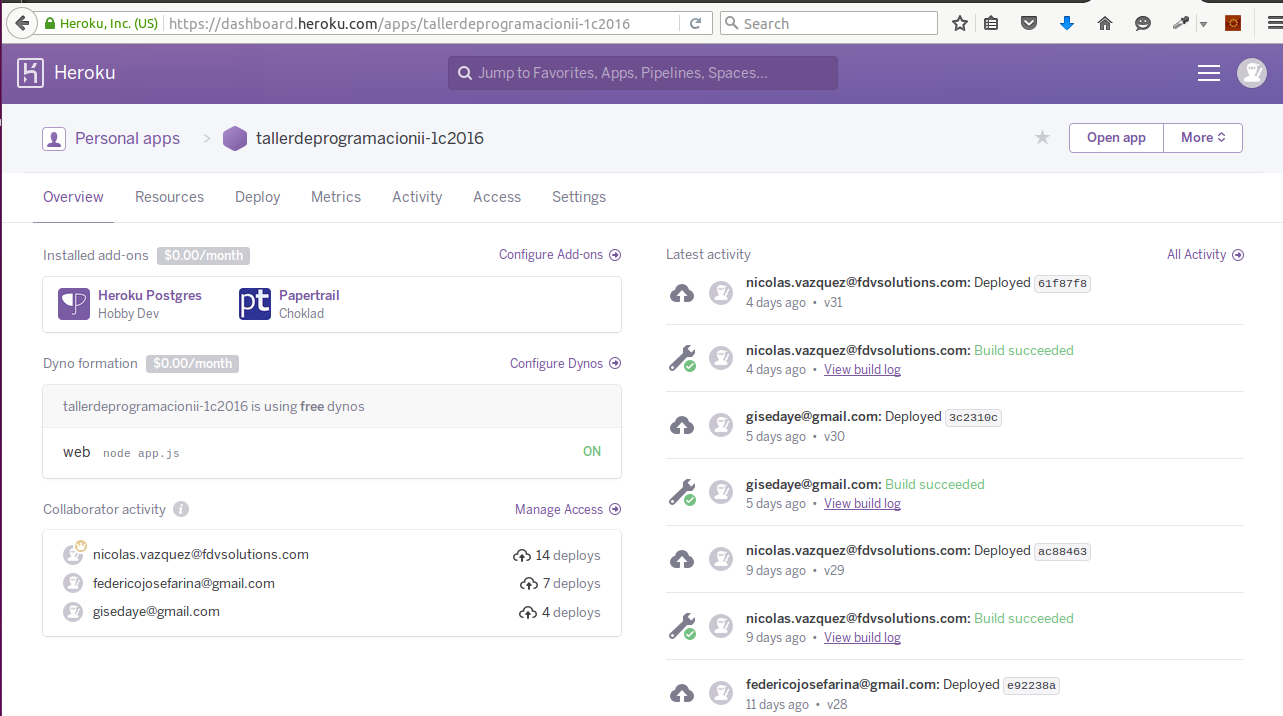
\includegraphics{heroku.png}
\begin{itemize}
\item {} 
Utilización de Express + Node.js en sus versiones 4.13 y 0.12.7 respectivamente.

\item {} 
Utilización de una base de datos PostgreSQL para almacenamiento de la información de Match App.

\end{itemize}

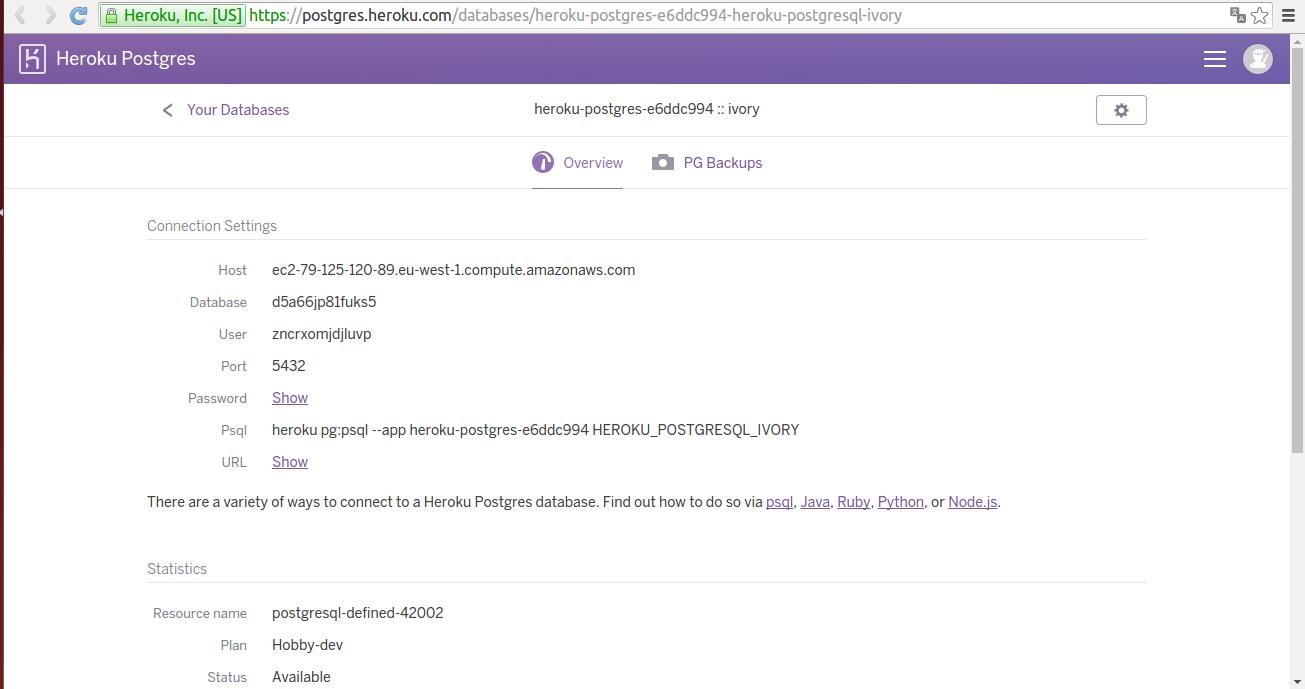
\includegraphics{postgresql.png}
\begin{itemize}
\item {} 
Aplicación Web utilizando CSS, HTML, Boostrap + Materialize, JQuery y Ajax.

\item {} 
Test  de endpoints con Postman

\item {} 
Docker

\end{itemize}


\subsection{Proyecto}
\label{manuals:proyecto}
-- Documentacion en Sphinx
- Repositorios git. Utilización de 3 repositorios en GitHub, uno para el cliente, otro para el App Server y otro para el Shared Server.
- Shared Server: \href{https://github.com/PabloFederico/SharedServer}{https://github.com/PabloFederico/SharedServer}
- App Server: \href{https://github.com/nicolas-vazquez/tp75521c}{https://github.com/nicolas-vazquez/tp75521c}
- Cliente y Documentación: \href{https://github.com/gisedaye/taller2android}{https://github.com/gisedaye/taller2android}


\section{Arquitectura}
\label{manuals:arquitectura}
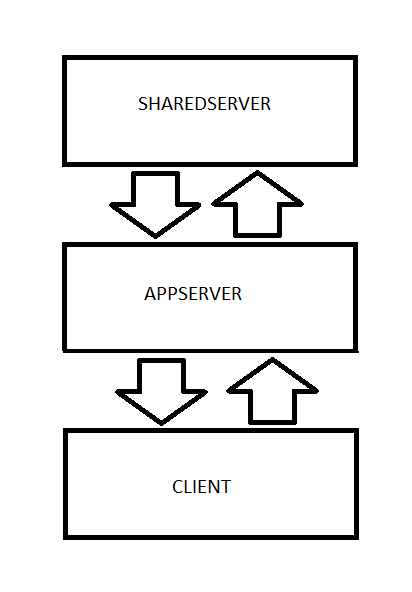
\includegraphics{architecture.png}


\subsection{Appserver}
\label{manuals:appserver}

\subsubsection{Esquemas}
\label{manuals:esquemas}
Paquetes del appServer

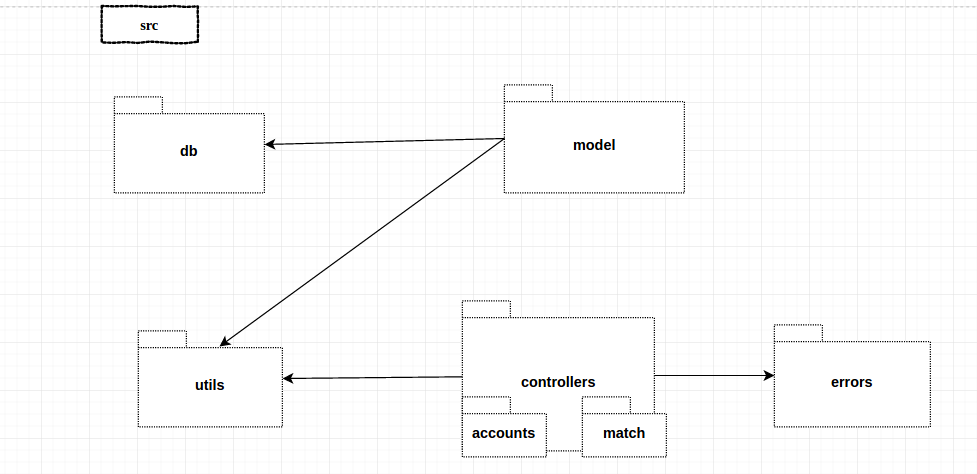
\includegraphics{paquetesApp.png}

Modelos y Controladores basicos del sistema.

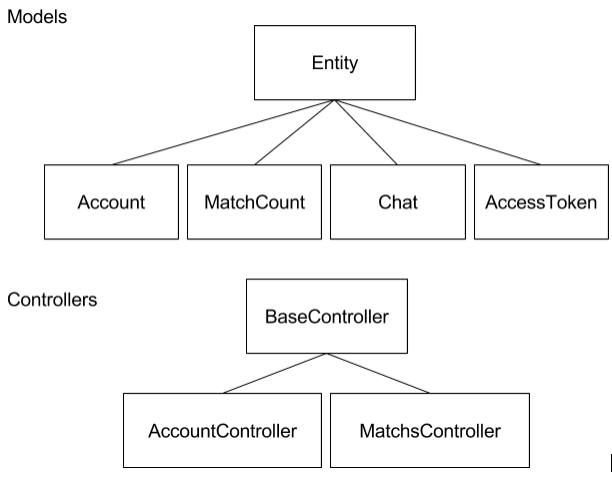
\includegraphics{classesapp.png}

Tablas de rocksDB con el contenido de sus registros.

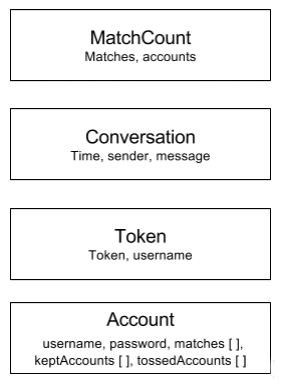
\includegraphics{rocksdb.png}

Diagrama de secuencia

..image:: Screenshots/secuenciaAppMain.png


\subsubsection{Endpoints}
\label{manuals:endpoints}
A continuacion se dara una breve descripcion de los distintos endpoints del appserver y como se manejan para obtener la informacion.


\subsubsection{Signup}
\label{manuals:signup}\begin{itemize}
\item {} 
Desde el cliente request a AppServer con los datos del profile y intereses completos.

\item {} 
Request a SharedServer para crear un usuario con los datos restantes (profile y intereses).

\item {} 
Guardo la información del profile en SharedServer.

\item {} 
El AppServer guarda username y password.

\item {} 
Vuelvo con un Successful SignUp all cliente.

\end{itemize}


\subsubsection{Login}
\label{manuals:login}\begin{itemize}
\item {} 
Desde el cliente request a AppServer con username/password

\item {} 
Busco el usuario en el AppServer:

\item {} 
En el caso que exista devuelvo accessToken

\item {} 
Si no existe hago un request a SharedServer, puede ser que el usuario haya sido creado desde el backoffice.

\item {} 
Busco el usuario en el SharedServer y devuelvo username/password

\item {} 
Guardo username/password y accesstoken/username en el AppServer

\item {} 
Vuelvo al cliente con el access token

\end{itemize}


\subsubsection{Like/Dislike}
\label{manuals:like-dislike}\begin{itemize}
\item {} 
Desde el cliente request a AppServer con el id

\item {} 
Guardamos el id en el array de keptAccounts

\item {} 
Si hay un match lo guardamos

\end{itemize}


\subsubsection{GetCandidates}
\label{manuals:getcandidates}\begin{itemize}
\item {} 
Desde el cliente request a AppServer  GET /candidates con location.

\item {} 
Busco el usuario en el AppServer, obtengo el username

\item {} 
Request a SharedServer con username

\item {} 
SharedServer determina los candidatos de acuerdo a los intereses del usuario

\item {} 
Devuelvo los candidatos al AppServer y filtro por likes/dislikes

\item {} 
Devuelvo los candidatos filtrados al cliente

\end{itemize}


\subsubsection{GetMatches}
\label{manuals:getmatches}\begin{itemize}
\item {} 
Desde el cliente request al AppServer GET /matches

\item {} 
Obtenemos la lista de matches

\item {} 
Request a SharedServer con la lista

\item {} 
Obtenemos los perfiles asociados

\item {} 
Devuelvo los matches al cliente

\end{itemize}


\subsection{Sharedserver}
\label{manuals:sharedserver}

\subsubsection{Esquemas}
\label{manuals:id1}\begin{itemize}
\item {} 
A continuación se mostrara un esquema de funcionamiento del Shared Sever, para poder explicar el flujo en la utilización de la api

\end{itemize}

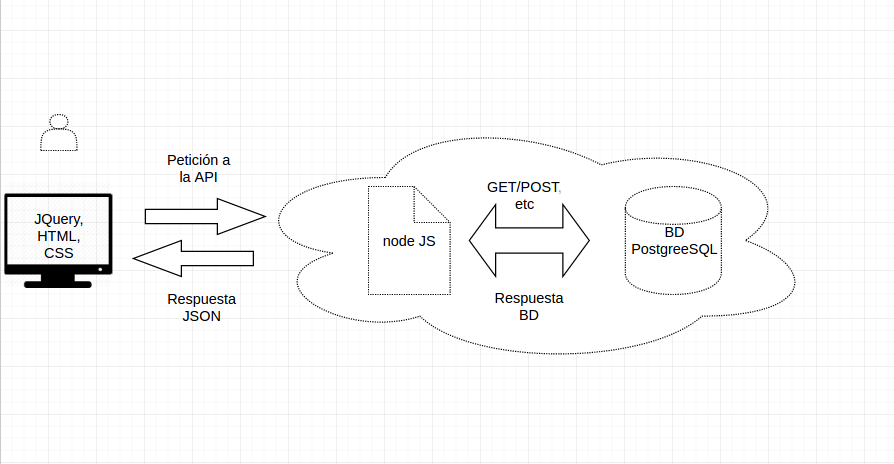
\includegraphics{esquemaShared.png}
\begin{itemize}
\item {} 
En el siguiente Diagrama de Componentes podemos visualizar la interacción entre los diferentes modulos de Shared Server. Por un lado, todas las librerias necesarias para el funcionamiento dentro de node\_modules, como estas son solicitadas por las vistas de la aplicación. La parte central del codigo comandado por el motor donde se encuentra el archivo inicial app.js y la intracción que éstos tienen con los otros componentes, como por ejemplo el node\_module

\end{itemize}

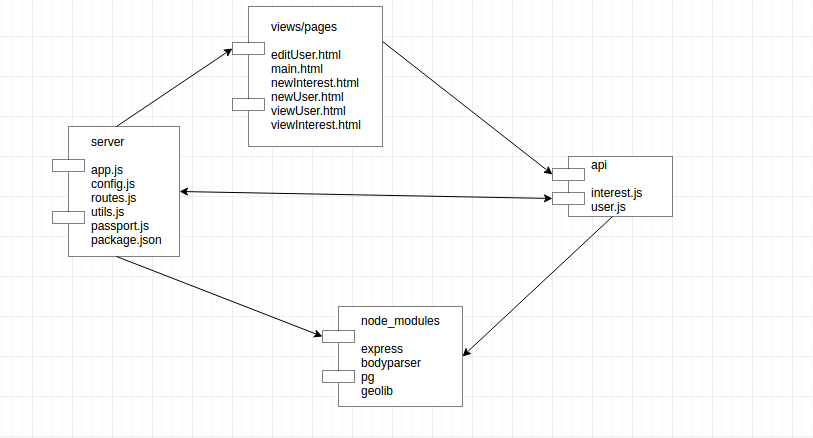
\includegraphics{componentes3Shared.png}
\begin{itemize}
\item {} 
Se crearon tres tablas en la base de datos de PostgreSQL para almacenar la información de los usuarios y sus intereses. EL esquema de tablas utilizados es el siguiente

\end{itemize}

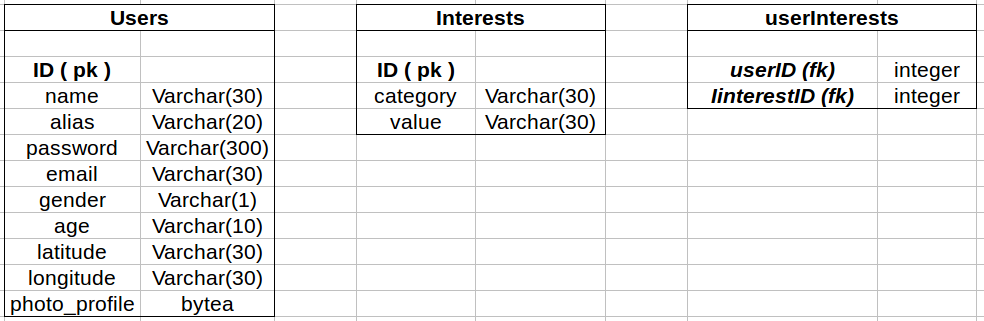
\includegraphics{tablasShared.png}
\begin{itemize}
\item {} 
El siguiente es un Diagrama Entidad-Relación utilizado:

\end{itemize}

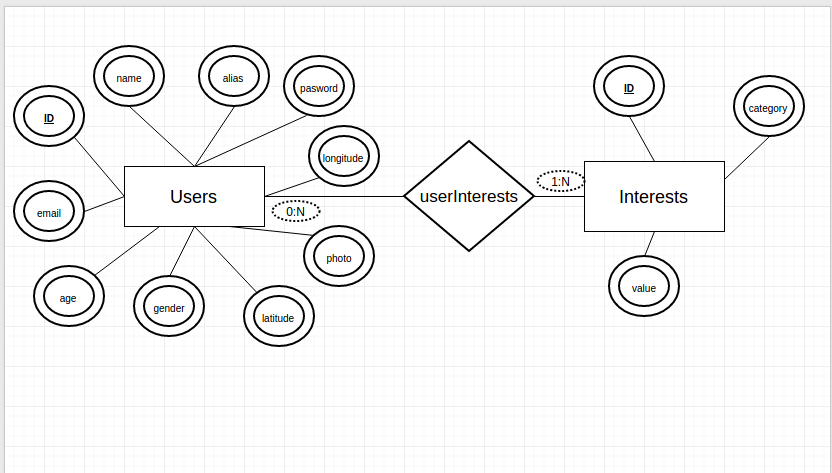
\includegraphics{derShared.png}


\subsubsection{Listado de usuarios}
\label{manuals:listado-de-usuarios}\begin{itemize}
\item {} 
Request GET /users/

\item {} 
Busca a todos los usuarios del sharedserver

\item {} 
Devuelve array de usuarios con: id, name, alias, email, sex, age, photo\_profile, array de interests, location, metadata

\end{itemize}


\subsubsection{Alta de usuario}
\label{manuals:alta-de-usuario}\begin{itemize}
\item {} 
Request POST /users/ con parametros: name, alias, email, sex, age, interests, location

\item {} 
Crea al usuario  en el sharedserver

\end{itemize}


\subsubsection{Consulta perfil de usuario}
\label{manuals:consulta-perfil-de-usuario}\begin{itemize}
\item {} 
Request GET /users/+id

\item {} 
Busca en el shared server usuario con ese id

\item {} 
Devuelve un objeto user con: id, name, alias, email, sex, age, photo\_profile, array de interests, location, metadata

\end{itemize}


\subsubsection{Edicion de usuario}
\label{manuals:edicion-de-usuario}\begin{itemize}
\item {} 
Request PUT /users/+id con parametros: id, name, alias, email, sex, age, photo\_profile, interests, location

\item {} 
Modifica al usuario  en el sharedserver

\end{itemize}


\subsubsection{Actualización foto perfil}
\label{manuals:actualizacion-foto-perfil}\begin{itemize}
\item {} 
Request PUT /users/+id/photo con parametro: photo en base64

\item {} 
Agrega una foto de perfil al usuario con id +id.

\end{itemize}


\subsubsection{Baja de usuario}
\label{manuals:baja-de-usuario}\begin{itemize}
\item {} 
Request DELETE /users/+id

\item {} 
Elimina al usuario del sharedserver

\end{itemize}


\subsubsection{Listado de intereses}
\label{manuals:listado-de-intereses}\begin{itemize}
\item {} 
Request GET /interests/

\item {} 
Busca a todos los intereses del sharedserver

\item {} 
Devuelve array de intereses con: category, value

\end{itemize}


\subsubsection{Alta de interes}
\label{manuals:alta-de-interes}\begin{itemize}
\item {} 
Request POST /interests/ con parametros: category, value

\item {} 
Crea al interes en el sharedserver en esa categoria

\end{itemize}


\subsection{Client}
\label{manuals:client}\begin{itemize}
\item {} 
Consume los endpoints del appserver para Login, Registro, Candidatos, Matches, Like, Dislike, Message, Messages, Users, Interests

\item {} 
Maneja session con el authorization token provisto por el endpoint del login

\item {} \begin{description}
\item[{Vistas:}] \leavevmode\begin{itemize}
\item {} 
LoginActivity

\item {} 
RegisterActivity

\item {} 
MainActivity

\item {} 
SplashActivity

\end{itemize}

\end{description}

\end{itemize}


\section{Testing}
\label{manuals:testing}

\subsection{Appserver}
\label{manuals:id2}

\subsubsection{Correr Unit Tests}
\label{manuals:correr-unit-tests}
En la consola desde la carpeta build ejecutar el comando
\begin{quote}

\textgreater{} ctest
\end{quote}


\subsubsection{Correr Coverage}
\label{manuals:correr-coverage}
En la raiz del proyecto correr
\begin{quote}

\textgreater{} sudo ./coverage.sh
\end{quote}

Se abrira una ventana del navegador con los resultados de tests cubiertos

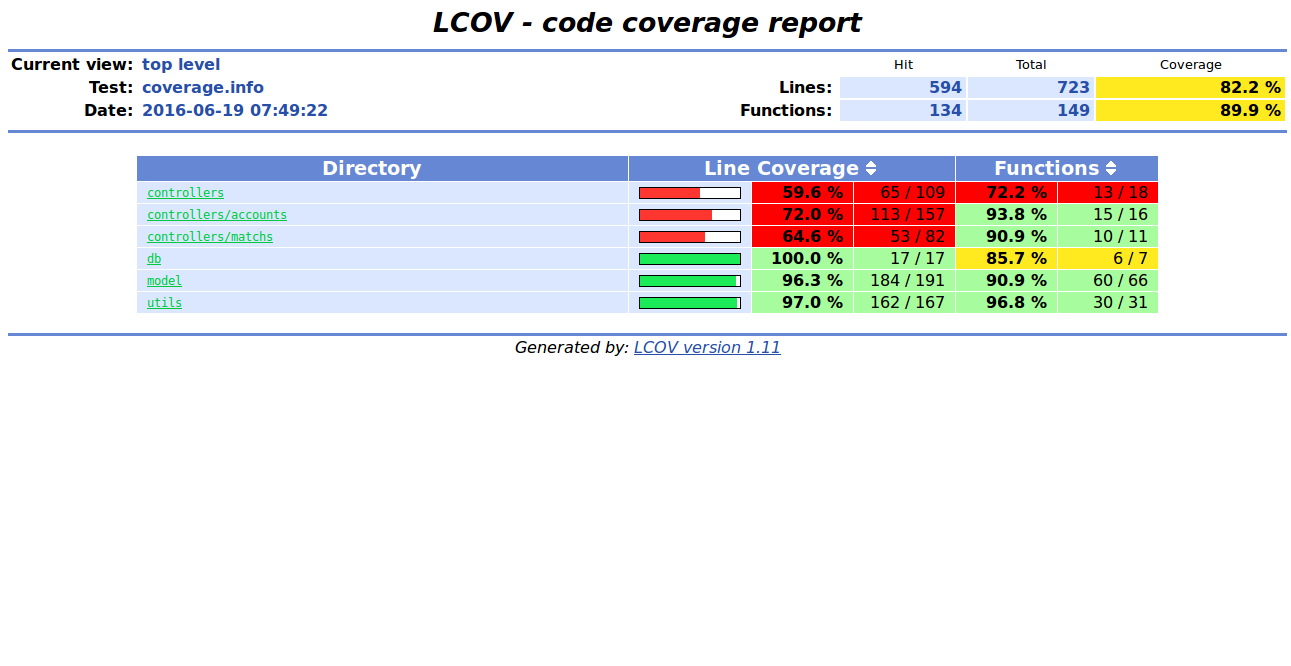
\includegraphics{coverage.png}


\subsubsection{Correr Tests funcionales}
\label{manuals:correr-tests-funcionales}
Instalar python

\textgreater{} sudo apt-get install python2.7

Instalar pip

\textgreater{} wget \href{https://bootstrap.pypa.io/get-pip.py}{https://bootstrap.pypa.io/get-pip.py}
\textgreater{} sudo python get-pip.py

Instalar el modulo requests

\textgreater{} sudo pip install requests

Para correr los tests funcionales ir al directorio functionalTests y correr los tests

\textgreater{} cd functionalTests/
\textgreater{} python python restTester.py

Saldran los resultados del tests en la consola


\subsubsection{Testear Endpoints Manualmente}
\label{manuals:testear-endpoints-manualmente}
Correr el appserver (Ver manual de instalacion)


\subsubsection{SignUp}
\label{manuals:id3}
\code{POST http://127.0.0.1:8083/api/accounts/signup}

En la tab body, seleccionar el radiobutton raw y agregar el siguiente texto

\code{\{
"username": "user",
"password": "P4ssw0rd"
\}}


\subsubsection{Login}
\label{manuals:id4}
\code{POST http://127.0.0.1:8083/api/accounts/login}

En la tab body, seleccionar el radiobutton raw y agregar el siguiente texto

\code{\{
"username": "user",
"password": "P4ssw0rd"
\}}


\subsubsection{Matches}
\label{manuals:matches}
\code{GET http://127.0.0.1:8083/api/matches/}

Agregar el header con el token que recibio del endpoint de login

\code{Authorization: \textless{}token\textgreater{}}


\subsubsection{Candidates}
\label{manuals:candidates}
\code{GET http://127.0.0.1:8083/api/matches/candidates/}

Agregar el header con el token que recibio del endpoint de login

\code{Authorization: \textless{}token\textgreater{}}


\subsubsection{Ver mensajes}
\label{manuals:ver-mensajes}
\code{GET http://127.0.0.1:8083/api/matches/1/messages/}

Agregar el header con el token que recibio del endpoint de login

\code{Authorization: \textless{}token\textgreater{}}


\subsubsection{Enviar mensaje}
\label{manuals:enviar-mensaje}
\code{PUT http://127.0.0.1:8083/api/matches/1/message/}

\code{\{
"message": "Hola!"
\}}

Agregar el header con el token que recibio del endpoint de login

\code{Authorization: \textless{}token\textgreater{}}


\subsubsection{Like}
\label{manuals:like}
\code{PUT http://127.0.0.1:8083/api/accounts/1/like/}

Agregar el header con el token que recibio del endpoint de login

\code{Authorization: \textless{}token\textgreater{}}


\subsubsection{Disike}
\label{manuals:disike}
\code{PUT http://127.0.0.1:8083/api/accounts/3/dislike/}

Agregar el header con el token que recibio del endpoint de login

\code{Authorization: \textless{}token\textgreater{}}


\subsection{Shared Server}
\label{manuals:id5}

\subsubsection{Login}
\label{manuals:id6}
\code{POST http://127.0.0.1:8083/api/accounts/login}

En la tab body, seleccionar el radiobutton raw y agregar el siguiente texto

\code{\{
"username": "user",
"password": "P4ssw0rd"
\}}

Agregar headers

\code{Authorization: \textless{}token\textgreater{}}
\code{Content-Type: application/json}


\subsubsection{Listado de  usuarios}
\label{manuals:id7}
\code{GET https://tallerdeprogramacionii-1c2016.herokuapp.com/users}


\subsubsection{Vista de un usuario}
\label{manuals:vista-de-un-usuario}
\code{GET https://tallerdeprogramacionii-1c2016.herokuapp.com/users/5}


\subsubsection{Vista de perfil de usuario}
\label{manuals:vista-de-perfil-de-usuario}
\code{GET https://tallerdeprogramacionii-1c2016.herokuapp.com/users/5/profile}

Agregar headers

\code{Authorization: \textless{}token\textgreater{}}
\code{Content-Type: application/json}


\subsubsection{Vista de candidatos de usuario}
\label{manuals:vista-de-candidatos-de-usuario}
\code{GET https://tallerdeprogramacionii-1c2016.herokuapp.com/users/nico/candidates}

Agregar headers

\code{Authorization: \textless{}token\textgreater{}}
\code{Content-Type: application/json}


\subsubsection{Alta de usuario}
\label{manuals:id8}
\code{POST https://tallerdeprogramacionii-1c2016.herokuapp.com/users}

\code{\{
"name":"Name",
"Alias":"aliiaass",
"email":"mail@mail.com",
"latitude":"21222",
"Longitude":"22322"
\}}


\subsubsection{Edit de usuario}
\label{manuals:edit-de-usuario}
\code{PUT https://tallerdeprogramacionii-1c2016.herokuapp.com/users/1}

\code{\{
"id": 1,
"name":"Name",
"Alias":"aliiaass",
"email":"mail@mail.com",
"latitude":"21222",
"Longitude":"22322"
\}}


\subsubsection{Baja de usuario}
\label{manuals:id9}
\code{DELETE https://tallerdeprogramacionii-1c2016.herokuapp.com/users/20}


\subsubsection{Listado de  intereses}
\label{manuals:id10}
\code{GET https://tallerdeprogramacionii-1c2016.herokuapp.com/interests}


\subsubsection{Alta de interes}
\label{manuals:id11}
\code{POST https://tallerdeprogramacionii-1c2016.herokuapp.com/interests}

\code{\{
"category":"Music",
"value":"One Direction"
\}}


\subsubsection{Baja de interes}
\label{manuals:baja-de-interes}
\code{DELETE https://tallerdeprogramacionii-1c2016.herokuapp.com/interests/2}


\chapter{Indices y tablas}
\label{index:indices-y-tablas}\begin{itemize}
\item {} 
\emph{genindex}

\item {} 
\emph{modindex}

\item {} 
\emph{search}

\end{itemize}



\renewcommand{\indexname}{Index}
\printindex
\end{document}
